\documentclass[a4paper,11pt,twoside]{report}
% Ajouter l'option 'pdf' lorsque vous compilez avec pdflatex
\usepackage[french]{babel}
\usepackage[utf8]{inputenc}
\usepackage{graphicx} 
\usepackage{float}
\usepackage{amsmath}
\newcommand{\norm}[1]{\left\lVert#1\right\rVert} %pour écrire une norme:  \norm{...}

\author{...}
\title{Reconnaissance de caractères}

\begin{document}
 
\maketitle 

%\begin{resume}
%...
%\end{resume}

\chapter{Introduction}
%MM

Le coeur du projet est d'écrire un code permettant de reconnaître automatiquement des caractères manuscrits, le but étant de se familiariser avec des méthodes usuelles de reconnaissance de forme en les implémentant pour un cas particulier et en en comprenant la théorie. \\


Les caractères à analyser seront ici des chiffres de 1 à 9 sous forme de vecteurs de taille $(28\times28,1)$ à valeurs entières comprise entre 0 et 255 : chaque vecteur représente une image de taille $28\times28$ en nuance de gris (0 = noir, blanc = 255). Nous disposons d'une base de données de 70000 chiffres manuscrits labellisés stockés sous le format décrit précédemment.\\
 
Nous avons choisi comme langage de programmation pour notre projet le Python.

\chapter{Pré-traitement des données}
La base de donnée étant un fichier matlab nous avons dans un premier temps du la traduire dans un format utilisable sous python. Nous avons choisi comme format de stockage une liste de liste de vecteurs : le $k^{eme}$ élément de cette liste est une liste des vecteurs correspondants au chiffre k.\\
Nous avons ensuite divisé la base de donnée en quatre afin que chacun des membre du groupe puisse effectuer des tests indépendants. 

Les algorithmes étudiés relèvent du domaine de l'apprentissage automatique : après une phase d'apprentissage où l'on donne à l'algorithme des images et les chiffres respectifs comme références, on a une phase de traitement où l'algorithme doit reconnaître le chiffre à partir de l'image seule. Pour avoir des résultats pertinents, il faut donc distinguer clairement les données utilisées pour l'apprentissage et celles utilisées pour le traitement.\\Le choix que nous avons fait est donc pour chaque base de donnée individuelle de diviser les données en $20\%$ fixe de données utilisées exclusivement pour les tests et de prendre pour donnée d'apprentissage aléatoirement $50\%$ des données restantes.




\chapter{Première méthode : calcul des écarts à la moyenne} 
\section{Théorie}
La première méthode étudiée est une approche assez intuitive du problème.\\
Dans un premier temps, à partir du set d’entraînement, pour chaque chiffre on crée une image moyenne de toutes les image du chiffre : le centre de gravité (centre de masse, isobarycentre) de tous les vecteurs de ce chiffre.\\Une image inconnue est alors classée en cherchant l'image moyenne telle que l'écart de ressemblance entre l'image à tester et cette image soit minimum.\\

On définit l'écart de ressemblance entre deux images comme étant la distance dans une certaine norme choisie entre les deux vecteurs $x$ et $y$ de $\textbf{R}^{784}$ correspondant aux images : $$d(x,y) = \norm{x-y}$$ Le choix de la norme et son influence sur les résultat est détaillé dans la partie pratique.

\section{Pratique}
Pour analyser l'efficacité de notre programme nous avons choisi d'observer deux types de données, le taux de réussite global de notre programme pour différentes normes, et le taux de réussite de notre programme pour chaque chiffre avec une norme fixe.\\
On a alors rapidement constaté grâce au graphe ci dessous, que les normes infini et 1 sont nettement moins efficaces que les autres, la norme la plus efficace semblant être la norme 3, puis on peut constater que l'efficacité  jusqu'à atteindre asymptotiquement celle de la norme infinie.\\%inserer graphique avec toutes les normes
% A discuter l'efficacité de la norme 3

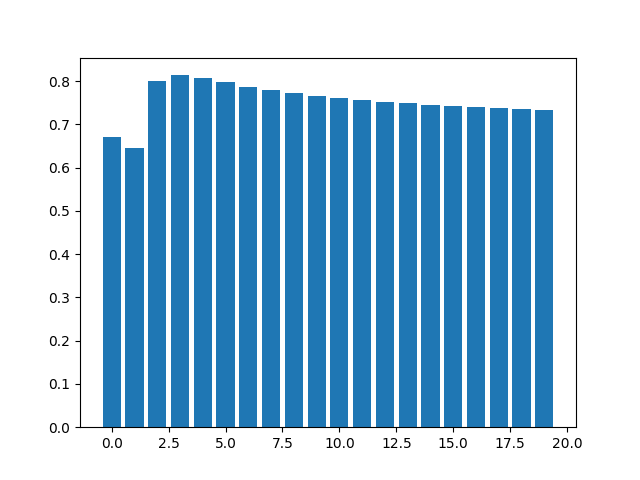
\includegraphics[scale=0.75]{Graphs/testNorme.png} \\



Pour essayer de comprendre ce résultat il est intéressant de regarder plus en détails sur quels chiffres notre programme échoue pour les normes 1,2 et infini.
% Discussion graphique / tableau
%insérer graphique de réussite pour les trois normes

%Idee? (si un des algorithmes a un temps de calcul eleve mais  est tres precise, faire une combinaison de algo simple avec seuil stricte + algo complexe pour les rejetées) + analyse 

%Inserer conclusion temporaire, meme si on modifie ulterieurement avec les resultats des autres, on peut faire un point sur le temps de calcul, et la relative efficacité de l'lagorithme.



\chapter{Deuxième méthode : utilisation de la décomposition en valeurs singulière (SVD)}
\subsection{Théorie}
Etant donné les résultats décevant de notre première méthode, il est nécessaire d'utiliser une autre technique qui prenne en compte les variations entre les différentes images représentant un même chiffre, cette technique repose sur un outil mathématique très puissant: la décomposition en matrices singulières (SVD).\\
Il s'agit ici dans un premier temps, de créer pour chaque chiffre (on parlera ici uniquement des trois pour alléger l'écriture) une matrice A de 784 lignes, comportant autant de colonnes que le nombre de 3 dont on dispose dans notre base d'entrainement. Chaque colonne de cette matrice représente une image de 3. On dispose alors d'un sous espace vectoriel de $\textbf{R}^{784}$ QUESTION: POURQUOI CET ESPACE EST DE FAIBLE DIMENSION?, engendré par les colonnes de A (on appelera cet espace vectoriel "l'espace des trois"). Or le théorème de décomposition en matrice singulière, nous permet de décomposer cette matrice ainsi: $$A = \sum_{i=1}^{784}{\sigma_{i}u_{i}v_{i}^{T}}$$\\
Les $u_{i}$ sont alors une base orthogonale de l'espace des trois. QUESTION: POURQUOI? De plus les la base peut être ordonné de manières à ce que les $\sigma_{i}$ forment une suite décroissante (ce qui est fait automatiquement sur les implémentation de base d'une SVD). Les premiers vecteurs de la SVD sont alors représentatif de l'espace vectoriel des 3, étant donné que toutes les matrices dans la somme sont de norme 1.\\
Maintenant qu'on dispose d'une base réduite de l'espace vectoriel des 3, on peut facilement calculer la distance pour la norme deux entre un chiffre non identifié (c'est à dire un vecteur de  $\textbf{R}^{784}$) et l'espace des 3 (cela revient à un calcul des moindres carrés). Si on effectue ce calcul pour l'espace correspondant à chaque chiffre on peut alors labélisé l'image, en constatant de quel espace vectoriel elle est le plus proche.

\subsection{Pratique}
\subsubsection{Clustering}%pourrait aller dans la partie pratique
Pour cette méthode, nous avons effectué une classification (clustering) plus fine des résultats : si lors de l'analyse d'une image, on ne peut l'identifier de façon décisive à un chiffre, celle-ci est rejetée, ce qui permet d'améliorer le taux d'identification correct parmi les images non rejetées. \\
Plus précisément, une image $z$ sera rejetée si le minimum $m1$ de l'ensemble des $ \norm{(I-U_{k}U_{k}^{T})z}_{2}$ (les moindres carrés pour chaque chiffre) n'est pas "significativement" plus petit que le deuxième plus petit élément de cet ensemble $m2$ (deux bases de chiffres pourraient alors correspondre à l'image). Pour définir ce "significativement" nous avons introduit un seuil compris entre $0.5$ et $1$ : une image sera rejetée si après le calcul de ses moindres carrés $m1>seuil*m2$. Plus le seuil est bas plus l'on est exigeant : avec un seuil de $1$ aucune image n'est rejetée et avec un seuil de $0.5$ l'évaluation d'une image est jugée concluante seulement si $m1\leq m2$.\\
\subsection{Paramètres}
Nous avons cherché à optimiser cette deuxième méthode en jouant sur deux paramètres : le nombre de vecteurs de base de $U$ choisis $k$ et le seuil.\\

%A revoir
Le premier set de test a été effectuée pour des valeurs du seuil entre 0.9 et 1 (des valeurs inférieures du seuil donnant un taux de rejet trop élevées env. 20\%) et une valeur de k (nombre de vecteurs de base) entre 1 et 7.\\

\begin{figure}[H]
  	\includegraphics[width=\linewidth]{"Graphs/3D TP vs Rejected".png}
  	\caption{A Modifier...}
\end{figure}

Le nombre de vecteurs de base $k$ choisi n'influe pas significativement sur la complexité des calculs : en effet seul le calcul de $I-U_{k}U_{k}^{T}$ dépend de $k$ et il est effectué une seule fois pour chaque chiffre. Cependant on remarque qu'au delà de 10 vecteurs de base, les résultats varient peu en fonction de $k$ %(cf.figure en haut 3D) 


Par la suite on fixe donc $k=10$.

\begin{figure}[H]
  	\includegraphics[width=\linewidth]{"Graphs/TP vs Rejected".png}
  	\caption{A Ajouter}
\end{figure}

	
On remarque dans les figures (numéro) le pourcentage de vrais positifs et le pourcentages de rejetés sont proportionnelles et linéairement décroissantes en fonction du seuil. On n'a donc pas de choix optimal objectif pour le seuil, on choisira donc le seuil en fonction de la tolérance à l'erreur et le taux de rejet acceptable. 


\chapter{Conclusion}

\bibliography{exemple} % Utilise exemple.bib
  
% Prints all the non-cited references
\nocite{*} 
% Use style 'alphakey' or 'alpha' for the draft, and then switch 
% to 'unsrt' or 'plain' or 'ieeetr' styles for the final version, 
% since they are the IEEE preferred ones. 
\bibliographystyle{ieeetr}
%\bibliographystyle{alpha}
\cleardoublepage

\appendix

\chapter{Annexe 1}
...
\end{document}
